% -*-coding: utf-8 -*-

%input "reference\reference.bib" % for winedt users
\def\version{a4-0.2}         % 哈尔滨工业大学硕博开题LaTeX模板

\def \xuewei {Doctor}     % 定义学位 博士
%\def \xuewei {Master}    % 硕士

\def\oneortwoside{twoside}% 双面打印 % oneside

\def\xueke{Engineering}   % 定义学科 工学
%\def\xueke{Science}      % 理学
%\def\xueke{Management}   % 管理学
%\def\xueke{Arts}         % 艺术学

\def\usewhat{xelatex}    % 你喜欢哪种编译方式,pdflatex dvipdfmx dvipspdf yap

\input{setup/type.tex}    % 硕博类型

%下面的book选项中可以使用 draft 选项,使插入的图形只显示外框,以加快预览速度。
\documentclass[12pt,a4paper,openany,\oneortwoside]{book}

%%%%%%%%%%%%%%%%%%%%%%%%%%%%%%%%%%%%%%%%%%%%%%%%%%%%%%%%%%%%%%%%%%%%%%%%%
%
%   LaTeX File for the Dissertation of Harbin Institute of Technology
%   LaTeX + CJK     ��������ҵ��ѧѧλ����ģ��
%   Based on Wang Lei's Template for Tsinghua University
%   Version: \beta
%   Last Update: 2004-04-28
%
%%%%%%%%%%%%%%%%%%%%%%%%%%%%%%%%%%%%%%%%%%%%%%%%%%%%%%%%%%%%%%%%%%%%%%%%%
%    by  Xiangqian Wu (HIT BBS: UFO, SMTH BBS: SuperUFO)
%                  csxqwu@hotmail.com
%%%%%%%%%%%%%%%%%%%%%%%%%%%%%%%%%%%%%%%%%%%%%%%%%%%%%%%%%%%%%%%%%%%%%%%%%
%%%%%%%%%%%%%%%%%%%%%%%%%%%%%%%%%%%%%%%%%%%%%%%%%%%%%%%%%%%%%%%%%%%%%%%%%
%
%   LaTeX File for Doctor (Master) Thesis of Tsinghua University
%   LaTeX + CJK     �廪��ѧ��ʿ��˶ʿ������ģ��
%   Based on Wang Tianshu's Template for XJTU
%   Version: 1.00
%   Last Update: 2003-09-12
%
%%%%%%%%%%%%%%%%%%%%%%%%%%%%%%%%%%%%%%%%%%%%%%%%%%%%%%%%%%%%%%%%%%%%%%%%%
%   Copyright 2002-2003  by  Lei Wang (BaconChina)       (bcpub@sina.com)
%%%%%%%%%%%%%%%%%%%%%%%%%%%%%%%%%%%%%%%%%%%%%%%%%%%%%%%%%%%%%%%%%%%%%%%%%

%%%%%%%%%%%%%%%%%%%%%%%%%%%%%%%%%%%%%%%%%%%%%%%%%%%%%%%%%%%%%%%%%%%%%%%%%
%
%   LaTeX File for phd thesis of xi'an Jiao Tong University
%
%%%%%%%%%%%%%%%%%%%%%%%%%%%%%%%%%%%%%%%%%%%%%%%%%%%%%%%%%%%%%%%%%%%%%%%%%
%   Copyright 2002  by  Wang Tianshu    (tswang@asia.com)
%%%%%%%%%%%%%%%%%%%%%%%%%%%%%%%%%%%%%%%%%%%%%%%%%%%%%%%%%%%%%%%%%%%%%%%%%

%%%%%%%%%%%%%%%%%%%%%%%%%%%%%%%%%%%%%%%%%%%%%%%%%%%%%%%%%%%
%
% Latex ������ͨ��ѧ��ʿ���ĵ�ģ��.
%
% ����ʹ��miktex2.1���װ�����ģ��
%
%%%%%%%%%%%%%%%%%%%%%%%%%%%%%%%%%%%%%%%%%%%%%%%%%%%%%%%%%%

%%%%%%%%%%%%%%%%%%%%%%%%%%%%%%%%%%%%%%%%%%%%%%%%%%%%%%%%%%%
%
% ���õĺ������Ӧ�Ķ���
%
%%%%%%%%%%%%%%%%%%%%%%%%%%%%%%%%%%%%%%%%%%%%%%%%%%%%%%%%%%%


% ͼ��֧�ֺ�� Ϊ��ʹ��pdftex ��Ҫ����Ӧ�ж�

%����һ�����ж�����
\newif\ifpdf
\ifx\pdfoutput\undefined
   \pdffalse
 \else
   \pdfoutput=1
   \pdftrue
 \fi



%%%%%%%%%%%%%%%%%%%   Modified By UFO   Begin  %%%%%%%%%%%%%%%%%%%%%%%
%%%%%%%��ɫ���ú���ǩ_UFO%%%%%%
\ifpdf
\usepackage[pdftex]{graphicx}

% ���ɴ���ǩ��pdf
\else
\usepackage[dvips]{graphicx}
\fi

%\usepackage[dvipdfm,
%            CJKbookmarks=true,
%            bookmarksnumbered=true,
%            bookmarksopen=true,
%            colorlinks=true,
%            pdfborder=001,
%            citecolor=blue,
%            linkcolor=red,
%            anchorcolor=green,
%            urlcolor=blue
%            ]{hyperref}
%%%%%%%%%%%%%%%%%%%   Modified By UFO   End  %%%%%%%%%%%%%%%%%%%%%%%%%

%

% ֧�ֲ�ɫ
\usepackage{color}
% epsͼ��
\usepackage{epsfig}

% �����������
\usepackage{indentfirst}

% ������ƺ��������涨�İ���ߴ�
%%%%%%%%%%%%%%%%%%%%%%%%%%
% HIT:
%���İ�о��Сһ��ӦΪ145mm��210mm������ҳü��ҳ����Ϊ145mm��230mm��
%ҳ���ڰ�о�±���֮�¸��о��з��ã�
%%%%%%%%%%%%%%%%%%%%%%%%%%
\usepackage[%paperwidth=18.4cm, paperheight= 26cm,
            body={14.5true cm,21true cm},
            twosideshift=0 pt,
            %headheight=1.0true cm
            ]{geometry}

% ����֧�ֺ��
\usepackage{CJK}

% ��ע����
\usepackage[perpage,symbol]{footmisc}

% AMSLaTeX��� �����ų�����Ư���Ĺ�ʽ
\usepackage{amsmath}
\usepackage{amssymb}

% ��ͬ��\mathcal or \mathfrak ֮���Ӣ�Ļ�������
\usepackage{mathrsfs}

% �����໷����������� amsmath ѡ���������� AMS LaTeX �ĺ��
\usepackage[amsmath,thmmarks]{ntheorem}

% ��Ϊͼ�οɸ�������ǰҳ�Ķ��������������ܻ����
% ���������ı���ǰ��. Ҫ��ֹ�����������ʹ�� flafter
% ���
%\usepackage{flafter}

%����ͼ�ο��ƺ��
%������һ��section�ĸ���ͼ�γ�������һ��section�Ŀ�ʼ����
%�ú���ṩ������������� \FloatBarrier ���ʹ����δ��
%���ĸ���ͼ������������
\usepackage[below]{placeins}

% ͼ�Ļ����ú��
\usepackage{floatflt}

% ͼ�κͱ���Ŀ���
\usepackage{rotating}

% tex1cm�������������Ĵ�С
\usepackage{type1cm}

% ���Ʊ���ĺ��
\usepackage[sf]{titlesec}

% ����Ŀ¼�ĺ��
%\usepackage{titletoc}
\usepackage{titletoc}
% ������ѧ��ʽ�еĺ�б��ĺ��
\usepackage{bm}

%�ɽ�����������õ��ļ������
%\usepackage{endfloat}

% fancyhdr��� ҳü��ҳ�ŵ���ض���
\usepackage{fancyhdr}
\usepackage{fancyref}

%%%%%%%%%%%%%%%%%%%   Modified By UFO   Begin  %%%%%%%%%%%%%%%%%%%%%%%

% ֧�����õĺ��
%\usepackage{cite}
% ֧��������д�ĺ��_UFO
\usepackage[sort&compress,numbers]{natbib}
\usepackage{hypernat}

%%%%%%%%%%%%%%%%%%%   Modified By UFO   End  %%%%%%%%%%%%%%%%%%%%%%%%%


%����ͼ�κͱ��������ʽ
\usepackage[centerlast]{caption2}

% ���Ʊ����ͼ�εĶ��б����о�
\usepackage{setspace}

% ��ӡ��ǰҳ���ʽ�ĺ��
\usepackage{layouts}

% ʹ��Times����ĺ��
\usepackage{times}

%%%%%%%%%%%%%%%%%%%   Added By UFO   Begin  %%%%%%%%%%%%%%%%%%%%%%%
%ʹ��Multirow�����ʹ�ñ�����Ժϲ����row��
\usepackage{multirow}
%֧����ͼ
\usepackage[hang, centerlast]{subfigure}
%��ѧ���
\usepackage{amsmath}
%%%%%%%%%%%%%%%%%%%   Added By UFO   End  %%%%%%%%%%%%%%%%%%%%%%%%%
\usepackage[dvipdfm,
            CJKbookmarks=true,
            bookmarksnumbered=true,
            bookmarksopen=true,
            colorlinks=true,
            pdfborder=001,
            citecolor=black,
            linkcolor=black,
            anchorcolor=black,
            urlcolor=black
            ]{hyperref}
\AtBeginDvi{\special{pdf:tounicode GBK-EUC-UCS2}} % GBK -> Unicode
\usepackage{hyperref}


\graphicspath{{figures/}} % 定义所有的eps文件在 figures 子目录下

\begin{document}
\zhspacing

%%%%%%%%%%%%%%%%%%%%%%%%%%%%%%%%%%%%%%%%%%%%%%%%%%%%%%%%%%%
% �ض�����������
% ע��win2000,û�� simsun,����õ�������һ��
% һЩ������office2000 ����
%%%%%%%%%%%%%%%%%%%%%%%%%%%%%%%%%%%%%%%%%%%%%%%%%%%%%%%%%%%
\newcommand{\song}{\CJKfamily{song}}    % ����   (Windows�Դ�simsun.ttf)
\newcommand{\fs}{\CJKfamily{fs}}        % ������ (Windows�Դ�simfs.ttf)
\newcommand{\kai}{\CJKfamily{kai}}      % ����   (Windows�Դ�simkai.ttf)
\newcommand{\hei}{\CJKfamily{hei}}      % ����   (Windows�Դ�simhei.ttf)
\newcommand{\li}{\CJKfamily{li}}        % ����   (Windows�Դ�simli.ttf)

%%%%%%%%%%%%%%%%%%%%%%%%%%%%%%%%%%%%%%%%%%%%%%%%%%%%%%%%%%%
% �ض����ֺ�����
%%%%%%%%%%%%%%%%%%%%%%%%%%%%%%%%%%%%%%%%%%%%%%%%%%%%%%%%%%%
\newcommand{\yihao}{\fontsize{26pt}{26pt}\selectfont}       % һ��, 1.���о�
\newcommand{\erhao}{\fontsize{22pt}{22pt}\selectfont}       % ����, 1.���о�
\newcommand{\xiaoer}{\fontsize{18pt}{18pt}\selectfont}      % С��, �����о�
\newcommand{\sanhao}{\fontsize{16pt}{16pt}\selectfont}      % ����, 1.���о�
\newcommand{\xiaosan}{\fontsize{15pt}{15pt}\selectfont}     % С��, 1.���о�
\newcommand{\sihao}{\fontsize{14pt}{14pt}\selectfont}       % �ĺ�, 1.0���о�
\newcommand{\banxiaosi}{\fontsize{13pt}{13pt}\selectfont}   % ��С��, 1.0���о�
\newcommand{\xiaosi}{\fontsize{12pt}{12pt}\selectfont}      % С��, 1.���о�
\newcommand{\dawuhao}{\fontsize{11.5pt}{11.5pt}\selectfont} % �����, �����о�
\newcommand{\wuhao}{\fontsize{10.5pt}{10.5pt}\selectfont}   % ���, �����о�
\newcommand{\xiaowu}{\fontsize{9.5pt}{9.5pt}\selectfont}    % ���, �����о�
\newcommand{\banbanxiaosi}{\fontsize{12pt}{12pt}\selectfont}% ���С��, 1.0���о�

%������ hyperref �� arydshln �����ݴ�����Ŀ¼����ʧЧ�����⡣
\def\temp{\relax}
\let\temp\addcontentsline
\gdef\addcontentsline{\phantomsection\temp}
\newcommand*{\subfigencaptionlist}{} % ��ͼ�μ���Ŀ¼ʱ��

\makeatletter
\gdef\hitfor{\@for}
\gdef\hitempty{}
\gdef\hittwo{\tw@}
\makeatother

\newcommand{\mr}[1]{\mathrm{#1}} %�����������\mr������\mathrm
\renewcommand\refname{��Ҫ�ο�����}
\renewcommand\bibname{��Ҫ�ο�����}

%����ͼ���½�˫��������
\newcommand{\figenname}{Fig.}
\newcommand{\listfigenname}{List of Figures}
\newfloatlist[chapter]{figen}{fen}{\listfigenname}{\figenname}
\newfixedcaption{\figencaption}{figen}
\renewcommand{\thefigen}{\arabic{figure}}
\makeatletter
\renewcommand{\@cftmakefentitle}{\chapter*{\listfigenname\@mkboth{\bfseries\listfigenname}{\bfseries\listfigenname}}}
\makeatother

\newcommand{\FigureBiCaption}[2] %˫�����
{\renewcommand{\figurename}{ͼ}
\vspace{-0.9ex}\caption{\protect\setlength{\baselineskip}{1.5em}#1} %\protect\setlength{\baselinestretch}{1.3}\selectfont
\vspace{-1.4ex}
\figencaption{\protect\setlength{\baselineskip}{1.5em}#2}%
%%����ͼ�μ���Ŀ¼
\makeatletter
\def\hittemp{}
 \hitfor \hittemp:=\subfigencaptionlist \do {%
        \ifx \hitempty\hittemp\relax \else
          \addcontentsline{fen}{subfigen}{\protect\numberline\hittemp}
        \fi}
 \gdef\subfigencaptionlist{}
\makeatother
}

\newcommand{\FigCaption}[1] %�������
{\renewcommand{\figurename}{ͼ}
\vspace{-0.9ex}\caption{\protect\setlength{\baselineskip}{1.5em}#1} %\protect\setlength{\baselinestretch}{1.3}\selectfont
}

\setcounter{fendepth}{2} %Ӣ��ͼ��Ŀ¼����� 1(ֻ��һ��Ŀ¼) 2(������Ŀ¼)
\setcounter{lofdepth}{2} %����ͼ��Ŀ¼����� 1(ֻ��һ��Ŀ¼) 2(������Ŀ¼)
\makeatletter
\renewcommand*{\l@subfigure}{\@dottedxxxline{\ext@subfigure}{2}{3.8em}{1.5em}} %����ͼ��Ŀ¼ subfigure
\gdef\l@subfigen{\@dottedtocline{0}{3.8em}{1.5em}}%Ӣ��ͼ��Ŀ¼ latex
\newif\ifsubfigtoc
\ifnum \tw@ > \@nameuse{c@fendepth} \subfigtocfalse \else \subfigtoctrue \fi
\makeatother
\newbox\tempbox
\newcommand{\SubfigEnCaption}[1]
{\makeatletter
 \ifsubfigtoc
    %����Ŀ¼���������һ��Ҫ�� ��ͼ ֮��,�������ݴ��� subfigencaptionlist
    \xdef\subfigencaptionlist{\subfigencaptionlist,%
        {{\thesubfigure}\protect\ignorespaces{#1}}}
\else
    \relax
\fi
\makeatother
%����caption
\vspace{-1.8ex}
\sbox{\tempbox}{\thesubfigure\hskip\subfiglabelskip #1}%
\ifthenelse{\lengthtest{\wd\tempbox > \linewidth}}%
{\\\parbox[t]{\linewidth}{\flushleft\noindent\CJKfamily{song}\rmfamily\xiaowu\selectfont\thesubfigure\hskip\subfiglabelskip #1\hangafter=1\hangindent=15pt}}%
{\\[2ex]\centerline{\CJKfamily{song}\rmfamily\xiaowu\selectfont\thesubfigure\hskip\subfiglabelskip #1}}
}

\newcommand{\tblenname}{Table} %define tbl instead of table
\newcommand{\listtblenname}{List of Tables}
\newfloatlist[chapter]{tblen}{ten}{\listtblenname}{\tblenname}
\newfixedcaption{\tblencaption}{tblen}
\renewcommand{\thetblen}{\arabic{table}}% ��tblen����table����Ϊtable��tablen���һ�£���tablen��\longbitoccaption��������Ч��
\makeatletter
\renewcommand{\@cftmaketentitle}{\chapter*{\listtblenname\@mkboth{\bfseries\listtblenname}{\bfseries\listtblenname}}}
\makeatother

\newcommand{\TableBiCaption}[2]%˫�����
{
\renewcommand{\tablename}{��}
\caption{\protect\setlength{\baselineskip}{1.5em}#1}
\vspace{-2ex}
\tblencaption{\protect\setlength{\baselineskip}{1.5em}#2}
\vspace{1ex}
}

\newcommand{\TabCaption}[1] %�������
{ \renewcommand{\tablename}{��}
  \caption{\protect\setlength{\baselineskip}{1.5em}#1}%
  \vspace{1.2ex}
}

%%%% �������caption����Ӣ�ı���Ŀ¼��������ʾ
\makeatletter
\def\@cont@LT@LTBiToeCaption#1[#2]#3{%
  \LT@makecaption#1\fnum@table{#3}%
  \def\@tempa{#2}%
  \ifx\@tempa\@empty\else
    {\let\\\space
      %\phantomsection
      \addcontentsline{ten}{tblen}{\protect\numberline{\thetable}{#2}}}%%\addcontentsline{lot}{table}{\protect\numberline{}{#2}}}%
  \fi}
\def\LT@c@ption#1[#2]#3{%
  \LT@makecaption#1\fnum@table{#3}%
  \def\@tempa{#2}%
  \ifx\@tempa\@empty\else
     {\let\\\space
     %\phantomsection
     \addcontentsline{lot}{table}{\protect\numberline{\thetable}{#2}}}%
  \fi}
\let\@cont@oldLT@c@ption\LT@c@ption
\newcommand*{\LTBiTocCaption}[5]{% ˫�����
  \@if@contemptyarg{#1}{\caption{#2}}{\caption[#1]{#2}}%
  \global\let\@cont@oldtablename\tablename
  \gdef\tablename{Table} %#3
  \global\let\LT@c@ption\@cont@LT@LTBiToeCaption
  \\
  \@if@contemptyarg{#4}{\caption{#5}}{\caption[#4]{#5}}%
  \global\let\tablename\@cont@oldtablename
  \global\let\LT@c@ption\@cont@oldLT@c@ption}
\makeatother

\makeatletter
\newcommand*{\LTCaption}[1]{ % �������
 \caption{#1}
}
\makeatother

\renewcommand{\cfttblendotsep}{1} %�Զ���ͼ��Ŀ¼�еĵ����С
\renewcommand{\cftfigendotsep}{1}

%%%---��ʽ�з�������----start----
%\begin{formulasymb}{ʽ��}{-3pt}%-3pt,-20pt�����Ϸ��ļ�ࡣ
%  \fdesfirst{��һ��ǩ}{���ƿ��ƿ��ƿ��ƿ���}
%  \fdes{������ǩ}{���ƿ��ƿ��ƿ��ƿ���}
%\end{formulasymb}
\newenvironment{formulades}[1]%
{\noindent\begin{list}{}{%
\setlength\topsep{0pt}
\settowidth{\labelwidth}{#1}
\setlength{\labelsep}{1mm}
\setlength{\leftmargin}{\labelwidth+\labelsep}
}}{\end{list}}
\newenvironment{formulasymb}[2]%-\!-\!-\!-
{\vspace*{#2}\newcommand{\fdesfirst}[2]%
{\begin{formulades}{#1\hspace*{22pt}##1~\cdash}\item[#1\hspace*{22pt}##1~\cdash]{##2}\end{formulades}\vspace*{-21pt}}%�Լ�����
\newcommand{\fdes}[2]{\begin{formulades}{#1\hspace{22pt}##1~\cdash}\item[##1~\cdash]{##2}\end{formulades}\vspace*{-21pt}}}%�Լ�����
{\vspace{21pt}\relax}%21pt����
%%----��ʽ�з�������----end-----

% ������BiChapter�� BiSection, ֱ�� Chapter Section .

\renewcommand{\thefigure}{\arabic{figure}}%ʹͼ���Ϊ 7-1 �ĸ�ʽ %\protect{~}
%\makeatletter
%\renewcommand\fnum@figure{\figurename\nobreakspace\thefigure\protect{~~~~~~~~~}} %
%\makeatother

\renewcommand{\thesubfigure}{\alph{subfigure})}%ʹ��ͼ���Ϊ a)�ĸ�ʽ
\makeatletter
\renewcommand{\p@subfigure}{\thefigure(} %%ʹ��ͼ����Ϊ 7-1(a) �ĸ�ʽ
\makeatother
%\renewcommand{\thesubfigure}{\alph{subfigure}}
%\makeatletter
%\renewcommand{\p@subfigure}{\thefigure} %%ʹ��ͼ����Ϊ 7-1a �ĸ�ʽ
%\renewcommand{\@thesubfigure}{\thesubfigure)\hskip\subfiglabelskip}%ʹ��ͼ���Ϊ a)�ĸ�ʽ
%\makeatother

\renewcommand{\thetable}{\arabic{table}}%%ʹ�����Ϊ 7-1 �ĸ�ʽ
\renewcommand{\theequation}{\arabic{equation}}%%ʹ��ʽ���Ϊ 7-1 �ĸ�ʽ

\setlength\jot{2.5ex}%���ù�ʽ֮��Ĵ�ֱ���� Ĭ��value = 3pt

%���� ѧ�� ѧλ
\def \xuekeEngineering {Engineering}
\def \xuekeScience {Science}
\def \xuekeManagement {Management}
\def \xuekeArts {Arts}

\ifx \xueke \xuekeEngineering
\newcommand{\cxueke}{��ѧ}
\newcommand{\exueke}{Engineering}
\fi

\ifx \xueke \xuekeScience
\newcommand{\cxueke}{��ѧ}
\newcommand{\exueke}{Science}
\fi

\ifx \xueke \xuekeManagement
\newcommand{\cxueke}{����ѧ}
\newcommand{\exueke}{Management}
\fi

\ifx \xueke \xuekeArts
\newcommand{\cxueke}{��ѧ}
\newcommand{\exueke}{Arts}
\fi

\newcommand{\cdash}{\mbox{��\!\!\!\!��\!\!\!\!��}}%�����������ۺŵ�����
\newcommand{\dif}{\mathrm{d}}%����ѧģʽ������΢��dx
  % 文本格式定义
% ���İ�о453.55pt��700.15pt,���մ� ftp://hitgs.hit.edu.cn/���صķ��棨20061211��
% ���õİ�о�����ܿ��ⱨ�治��װ�������԰�о�Ȳ�ʿ���Ĵ�
% ҳ���ڰ�о�±���֮�¸��о��з��ã�
% ����
\setlength{\textwidth}{453.55pt}      % �ı�����
\setlength{\oddsidemargin}{0pt}   % ��� 3.25cm=0.71+2.54 % ��߾�
\setlength{\evensidemargin}{0pt}
%  ����
\setlength{\topmargin}{-32pt}       % 3.3=2.54+0.76  ҳ�� ���¶� 0.42
\setlength{\headheight}{20pt}      % 0.8  ҳü�߶�
\setlength{\headsep}{10pt}         % 0.4
\setlength{\textheight}{700.15pt}     % 21.0  �ı��߶�
\setlength{\footskip}{26pt}        %1.1  ����ҳ��
%%%%%%%%%%%%%%%%%%%%%%%%%%%%%%%%%%%%%%%%%%%%%%%%%%%%%%%%%%%
%������ʽ��ҳ��ʾ,��������Ƶ���ʽ����һҳ�ڣ�
%һҳ��ʾ���·ŵ��ڶ�ҳ�����ºܴ�Ŀհ׿ռ䣬�ܲ��ÿ�
\allowdisplaybreaks[4]

%%%%%%%%%%%%%%%%%%%%%%%%%%%%%%%%%%%%%%%%%%%%%%%%%%%%%%%%%%%
%������������ʹ���������ȱʡֵ��΢����һ�㣬�Ӷ���ֹ����
%����ռ�ݹ�����ı�ҳ�棬Ҳ���Է�ֹ�ںܴ�հ׵ĸ���ҳ�Ϸ��ú�С��ͼ�Ρ�
\renewcommand{\topfraction}{0.9999999}
\renewcommand{\textfraction}{0.0000001}
\renewcommand{\floatpagefraction}{0.9999}

%%%%%%%%%%%%%%%%%%%%%%%%%%%%%%%%%%%%%%%%%%%%%%%%%%%%%%%%%%%
% �ض���һЩ������ر���
%%%%%%%%%%%%%%%%%%%%%%%%%%%%%%%%%%%%%%%%%%%%%%%%%%%%%%%%%%%
\theoremstyle{plain} \theorembodyfont{\song\rmfamily}
\theoremheaderfont{\hei\rmfamily} %\theoremseparator{:}
\newtheorem{definition}{\hei ����}[chapter]
\newtheorem{proposition}[definition]{\hei ����}
\newtheorem{lemma}[definition]{\hei ����}
\newtheorem{theorem}{\hei ����}[chapter]
\newtheorem{axiom}{\hei ����}
\newtheorem{corollary}[definition]{\hei ����}
\newtheorem{exercise}[definition]{}

%%%%%%%%%%%%%%%%%%%%%%%%%%%%%%%%%%%%%%%%%%%%%%%%%%%%%%%%%%%%%%%%%%%
%���ԭproof�����������������⣺
%  1. proof �е�item��������
%  2. proof �е����һ����ʽ�³���һ���ڷ��顣
%\theoremsymbol{$\blacksquare$}
%\newtheorem{proof}{\hei ֤��}
\newenvironment{proof}{\noindent{\hei ֤����}}{\hfill $ \square $ \vskip 4mm}
\theoremsymbol{$\square$}
\newtheorem{example}{\hei ��}

%%%%%%%%%%%%%%%%%%%%%%%%%%%%%%%%%%%%%%%%%%%%%%%%%%%%%%%%%%%
% �������Ķ������� �����İ�ʽ
%%%%%%%%%%%%%%%%%%%%%%%%%%%%%%%%%%%%%%%%%%%%%%%%%%%%%%%%%%%
%\CJKcaption{GB_aloft}
\CJKcaption{gb_452}

\newlength \CJKtwospaces

\def\CJKindent{
    \settowidth\CJKtwospaces{\CJKchar{"0A1}{"0A1}\CJKchar{"0A1}{"0A1}}%
    \parindent\CJKtwospaces
}

\CJKtilde  \CJKindent

\setlength{\parindent}{26pt} %���ڹ������ĵ�ÿ�е��־�Ӵ��ˣ���Ҫ���Ӷ�����2pt

\renewcommand\contentsname{\hei Ŀ~~~~¼}

%%%%%%�½ڱ���Ϊ����1�¡�����ʽ
\renewcommand\chaptername{}%��
%%%%%%%%%%%%%%%%%%%%%%%%%%%%%%%%%%%%%%%%%%%%%%%%%%
%��������½ڵı����Ŀ¼��ĸ�ʽ
%%%%%%%%%%%%%%%%%%%%%%%%%%%%%%%%%%%%%%%%%%%%%%%%%%
\setcounter{secnumdepth}{4} \setcounter{tocdepth}{2}

\titleformat{\chapter}[hang]{\xiaoer\bf\filcenter\hei\sf\boldmath}{\xiaoer\chaptertitlename}{18pt}{\xiaoer}
\titlespacing{\chapter}{0pt}{8pt}{16pt}

\titleformat{\section}[hang]{\hei\sf\xiaosan\boldmath}{\xiaosan\thesection}{0.5em}{}
\titlespacing{\section}{0pt}{13pt}{13pt}
\makeatletter
\renewcommand\thesection{\@arabic \c@section} % ǰ�治�� thechapter
\makeatother

\titleformat{\subsection}[hang]{\hei\sf\sihao\boldmath}{\sihao\thesubsection}{0.5em}{}
\titlespacing{\subsection}{0pt}{8pt}{7pt}

\titleformat{\subsubsection}[runin]{\hei\sf\xiaosi\boldmath}{\thesubsubsection}{0.5em}{}[\;\;]
%\titleformat{\subsubsection}[hang]{\hei\sf\xiaosi}{\xiaosi\thesubsubsection}{0.5em}{}
\titlespacing{\subsubsection}{0pt}{3pt}{2pt}   % #2�����ļ�� #3�����ļ��

%��������Ŀ¼,����û��Ŀ¼
%\dottedcontents{chapter}[3.4em]{\vspace{0.5em}\hspace{-3.4em}\hei \bf\boldmath}{0.0em}{5pt}
%\dottedcontents{section}[1.16cm]{}{1.8em}{5pt}
%\dottedcontents{subsection}[2.00cm]{}{2.7em}{5pt}
%\dottedcontents{subsubsection}[2.86cm]{}{3.4em}{5pt}

%%%%%%%%%%%%%%%%%%%%%%%%%%%%%%%%%%%%%%%%%%%%%%%%%%%%%%%
% ����ҳü��ҳ�� ʹ��fancyhdr ���
%%%%%%%%%%%%%%%%%%%%%%%%%%%%%%%%%%%%%%%%%%%%%%%%%%%%%%%%
\newcommand{\makeheadrule}{%
\makebox[-3pt][l]{\rule[.7\baselineskip]{\headwidth}{0.4pt}}
\rule[0.85\baselineskip]{\headwidth}{2.25pt}\vskip-.8\baselineskip}
\makeatletter
\renewcommand{\headrule}{%
    {\if@fancyplain\let\headrulewidth\plainheadrulewidth\fi
     \makeheadrule}}

\pagestyle{fancyplain}

%ȥ���½ڱ����е�����
%%��Ҫע����һ�У�����ҳü���ɣ�����1��1  ���ۡ���ʽ
\renewcommand{\chaptermark}[1]{\markboth{\chaptertitlename~~ \ #1}{}}
 \fancyhf{}

%��book�ļ������,\leftmark�Զ���¼����֮����,\rightmark��¼�ڱ���
%% ҳü�ֺ� ����Ҫ�� С��
%���ݵ�˫���ӡ���ò�ͬ��ҳü��
\ifoneortwoside
  \fancyhead[CO]{\CJKfamily{song}\xiaowu\rightmark}
  \fancyhead[CE]{\CJKfamily{song}\xiaowu ��������ҵ��ѧ\cxueke\cxuewei ѧλ���Ŀ��ⱨ��}% ����ҳü����ߵľ���
  \fancyfoot[C,C]{\xiaowu\thepage}
\else
  \fancyhead[CO]{\CJKfamily{song}\xiaowu ��������ҵ��ѧ\cxueke\cxuewei ѧλ���Ŀ��ⱨ��}
  \fancyhead[CE]{\CJKfamily{song}\xiaowu ��������ҵ��ѧ\cxueke\cxuewei ѧλ���Ŀ��ⱨ��}% ����ҳü����ߵľ���
  \fancyfoot[C,C]{\xiaowu\thepage}
\fi

%%%%%%%%%%%%%%%%%%%%%%%%%%%%%%%%%%%%%%%%%%%%%%%%%%%%%%%%
% �����о�Ͷ���䴹ֱ����
%%%%%%%%%%%%%%%%%%%%%%%%%%%%%%%%%%%%%%%%%%%%%%%%%%%%%%%%
\renewcommand{\CJKglue}{\hskip 0.3pt plus 0.08\baselineskip}%�Ӵ��ּ�࣬ʹÿ��33����
%\setlength{\belowcaptionskip}{10pt}   % �Ӵ����ͱ���֮��ľ���
\setlength{\parskip}{3pt plus1pt minus1pt} % ����֮�����ֱ����
\renewcommand{\baselinestretch}{1.2}% �����о�

%%%%%%%%%%%%%%%%%%%%%%%%%%%%%%%%%%%%%%%%%%%%%%%%%%%%%%%%
% �����б������Ĵ�ֱ���
%%%%%%%%%%%%%%%%%%%%%%%%%%%%%%%%%%%%%%%%%%%%%%%%%%%%%%%%
\setitemize{itemindent=38pt,leftmargin=0pt,itemsep=-0.4ex,listparindent=26pt,partopsep=0pt,parsep=0.5ex,topsep=-0.25ex}
\setenumerate{itemindent=38pt,leftmargin=0pt,itemsep=-0.4ex,listparindent=26pt,partopsep=0pt,parsep=0.5ex,topsep=-0.25ex}
\setdescription{itemindent=38pt,leftmargin=0pt,itemsep=-0.4ex,listparindent=26pt,partopsep=0pt,parsep=0.5ex,topsep=-0.25ex}

%%�����
\renewcommand\bibsection{\section*{\centerline{\refname}}\vspace{-6pt}\markboth{��������ҵ��ѧ\cxueke\cxuewei ѧλ���Ŀ��ⱨ��}{\refname}} %���У������ļ��
\renewcommand\@biblabel[1]{[#1]\hspace{0.5em}} %�ο������������ߵ�����
\newcommand{\ucite}[1]{$^{\mbox{\scriptsize \cite{#1}}}$} % ���� \ucite ����ʹ��ʾ������Ϊ�ϱ���ʽ
\newcommand{\citeup}[1]{$^{\mbox{\scriptsize \cite{#1}}}$} % for WinEdt users

%%%%%%%%%%%%%%%%%%%%%%%%%%%%%%%%%%%%%%%%%%%%%%%%%%%%%%%%%%%
% ���Ƹ���ͼ�κͱ��������ʽ %������ccaption��ȫ������caption2�Ĺ���
\captionstyle{\centering}   %��ͬ��ͼ������ʽ���ò�ͬ������
%\indentcaption{0pt}           %�μ�ccaption
\hangcaption
\captionnamefont{\CJKfamily{song}\rmfamily\wuhao\selectfont}
\captiontitlefont{\CJKfamily{song}\rmfamily\wuhao\selectfont}
\captiondelim{~} %~

%%%%%%%%%%%%%%%%%%%%%%%%%%%%%%%%%%%%%%%%%%%%%%%%%%%%%%%
% ������ͷ���Եĸ�ʽ
% �÷� \begin{Aphorism}{author}
%         aphorism
%      \end{Aphorism}
\newsavebox{\AphorismAuthor}
\newenvironment{Aphorism}[1]
{\vspace{0.5cm}\begin{sloppypar} \slshape
\sbox{\AphorismAuthor}{#1}
\begin{quote}\small\itshape }
{\\ \hspace*{\fill}------\hspace{0.2cm} \usebox{\AphorismAuthor}
\end{quote}
\end{sloppypar}\vspace{0.5cm}}

%�Զ���һ�����������ע�͵��ı��в���Ҫ�IJ��֡�
\newcommand{\comment}[1]{}

\renewcommand\contentsname{\hei Ŀ~~~~¼}
\renewcommand\listfigurename{\hei ��~~~~ͼ}
\renewcommand\listtablename{\hei ��~~~~��}

%%%%%%���±����е��������֣�һ������������Ϊ����������(1,2,3)
\renewcommand\CJKthechapter{%\CJKnumber
{\@arabic\c@chapter}}

%%%%%%��Ҫ�����о�ʹ��ҳ�����
\raggedbottom

% This is the flag for longer version
\newcommand{\longer}[2]{#1}
\newcommand{\ds}{\displaystyle}
% define graph scale
\def\gs{1.0}

%%%%%%%%%%%%%%%%%%%%%%%%%%%%%%%%%%%%%%%%%%%%%%%%%%%%%%%%%%%%%%%%%%%%%%
% �Զ�����Ŀ�б���ǩ����ʽ \begin{hitlist} �б��� \end{hitlist}
%%%%%%%%%%%%%%%%%%%%%%%%%%%%%%%%%%%%%%%%%%%%%%%%%%%%%%%%%%%%%%%%%%%%%%
\newcounter{hitctr} %�Զ����¼�����
\newenvironment{hitlist}{%%%%%�����»���
\begin{list}{{\hei (\arabic{hitctr})}} %%��ǩ��ʽ
    {
     \usecounter{hitctr}
     \setlength{\leftmargin}{0cm}     %��߽�
     \setlength{\parsep}{0ex}         %������
     \setlength{\topsep}{0pt}         %�б��������ĵĴ�ֱ����
     \setlength{\itemsep}{0ex}        %��ǩ���
     \setlength{\labelsep}{0.3em}     %��ź��б���֮��ľ���,Ĭ��0.5em
     \setlength{\itemindent}{46pt}    %��ǩ������
     \setlength{\listparindent}{27pt} %����������
    }}
{\end{list}}%%%%%

%%%%%%%%%%%%%%%%%%%%%%%%%%%%%%%%%%%%%%%%%%%%%%%%%%%%%%%%%%%%%%%%%%%%%%
% �Զ�����Ŀ�б���ǩ����ʽ \begin{publist} �б��� \end{publist}
%%%%%%%%%%%%%%%%%%%%%%%%%%%%%%%%%%%%%%%%%%%%%%%%%%%%%%%%%%%%%%%%%%%%%%
\newcounter{pubctr} %�Զ����¼�����
\newenvironment{publist}{%%%%%�����»���
\begin{list}{\arabic{pubctr}} %%��ǩ��ʽ
    {
     \usecounter{pubctr}
     \setlength{\leftmargin}{2em}     % ��߽� \leftmargin =\itemindent + \labelwidth + \labelsep
     \setlength{\itemindent}{0em}     % ���������
     \setlength{\labelwidth}{1em}     % ��ſ���
     \setlength{\labelsep}{1em}       % ��ź��б���֮��ľ���,Ĭ��0.5em
     \setlength{\rightmargin}{0em}    % �ұ߽�
     \setlength{\topsep}{0ex}         % �б��������ĵĴ�ֱ����
%     \setlength{\partopsep}{0ex}      % �б���һ���µĶ���ʱ���ӵĶ��⵽�����ĵľ���
     \setlength{\parsep}{0ex}         % ������
     \setlength{\itemsep}{0ex}        % ��ǩ���
     \setlength{\listparindent}{26pt} % ����������
    }}
{\end{list}}%%%%%

%%%%%%%%%%%%%%%%%%%%%%%%%%%%%%%%%%%%%%%%%%%%%%%%%%%%%%%%%%%%%%%%%%%%%%
% Ĭ������
\renewcommand\normalsize{%
  \@setfontsize\normalsize{12.1pt}{13pt}
  \setlength\abovedisplayskip{10pt plus 2pt minus 2pt}
  \setlength\abovedisplayshortskip{8pt plus 2pt minus 2pt}
  \setlength\belowdisplayskip{\abovedisplayskip}
  \setlength\belowdisplayshortskip{\abovedisplayshortskip}
  \setlength\jot{8pt}
  \let\@listi\@listI}
\def\defaultfont{\renewcommand{\baselinestretch}{1.37}\normalsize\selectfont}

%%%%%%%%%%%%%%%%%%%%%%%%%%%%%%%%%%%%%%%%%%%%%%%%%%%%%%%%%%%%%%%%%%%%%%
% ���桢ժҪ����Ȩ����л��ʽ����
\makeatletter
\def\caffil#1{\def\@caffil{#1}}\def\@caffil{}
\def\csubject#1{\def\@csubject{#1}}\def\@csubject{}
\def\csupervisor#1{\def\@csupervisor{#1}}\def\@csupervisor{}
\def\cassosupervisor#1{\def\@cassosupervisor{~ & {\textbf{��\hfill ��\hfill ʦ}}& \rule[-3pt]{201pt}{1.2pt}\hspace{-201pt}\centerline{#1}\\[16pt]}}\def\@cassosupervisor{}
\def\cauthor#1{\def\@cauthor{#1}}\def\@cauthor{}
\def\cbdate#1{\def\@cbdate{#1}}\def\@cbdate{} %��ѧʱ��
\def\cdate#1{\def\@cdate{#1}}\def\@cdate{}    %��������
\def\ctitle#1{\def\@ctitle{#1}}\def\@ctitle{}
\def\ctitlesec#1{\def\@ctitlesec{~ & ~ & \rule[-3pt]{201pt}{1.2pt}\hspace{-201pt}\centerline{#1}}}\def\@ctitlesec{}
%%%%%%%%%%%%%%%%%%%%%%%%%%%%%%%%%%%%%%%%%%%%%%%%%%%%%%%%%%%%%%%
% �������
\ifxueweidoctor
\def\makecover{ \normalbiao
    \setboolean{@twoside}{true}
    %%%%%%%%%%%%%����һ
    \thispagestyle{empty}
    \vspace*{42pt}
    \begin{center}
    {\kai\xiaoer \makebox[152pt][s]{\textbf{��������ҵ��ѧ}}}
    \end{center}

    \vspace{16pt}
    \begin{center}
      {\song\erhao\makebox[258pt][c]{\textbf{\xueweishort\hfill ʿ\hfillѧ\hfillλ\hfill��\hfill��\hfill��\hfill��\hfill��\hfill��}}}
    \end{center}

    \vspace{64.8pt}
    {\song\sanhao
    \def\oldtabcolsep{\tabcolsep}
    \setlength{\tabcolsep}{0pt}
    \noindent\begin{tabular}{p{69pt}p{97pt}p{201pt}lll}\setlength{\tabcolsep}{-30pt}
    ~ & {\textbf{Ժ\hfill (ϵ)}}                                   & \rule[-3pt]{201pt}{1.2pt}\hspace{-201pt}\centerline{\@caffil}\\[16pt]
    ~ & {\textbf{ѧ\hfill ��}}                                     & \rule[-3pt]{201pt}{1.2pt}\hspace{-201pt}\centerline{\@csubject}\\[16pt]
    ~ & {\textbf{��\hfill ʦ}}                                     & \rule[-3pt]{201pt}{1.2pt}\hspace{-201pt}\centerline{\@csupervisor}\\[16pt]
    \@cassosupervisor
    ~ & {\textbf{��\hfill ��\hfill ��}}                            & \rule[-3pt]{201pt}{1.2pt}\hspace{-201pt}\centerline{\@cauthor}\\[16pt]
    ~ & {\textbf{��\hfill ѧ\hfill ʱ\hfill ��}}                   & \rule[-3pt]{201pt}{1.2pt}\hspace{-201pt}\centerline{\@cbdate}\\[16pt]
    ~ & {\textbf{��\hskip-0.4pt\hfill ��\hskip-0.4pt\hfill ��\hskip-0.4pt\hfill ��\hskip-0.4pt\hfill ��\hskip-0.4pt\hfill ��}} & \rule[-3pt]{201pt}{1.2pt}\hspace{-201pt}\centerline{\@cdate}\\[16pt]
    ~ & {\textbf{��\hfill ��\hfill ��\hfill Ŀ}}                   & \rule[-3pt]{201pt}{1.2pt}\hspace{-201pt}\centerline{\@ctitle}\\[16pt]
    \@ctitlesec
    \end{tabular}
    \def\tabcolsep{\oldtabcolsep}
    \vspace{154pt}
    \begin{center}
    \textbf{�о���Ժ������}
    \end{center}
}

%%�����ڷ�
\newpage
\thispagestyle{empty}
\vspace*{14pt}
\begin{center}
  {\hei\sanhao \makebox[85pt][s]{˵\hfill ��}}
\end{center}
\vspace*{40pt}
    {\song\renewcommand\baselinestretch{1.27}
    \fontsize{10.5pt}{12.6pt}\selectfont
    \noindent һ�����ⱨ��Ӧ����������Ҫ���ݣ�
    \begin{enumerate}[leftmargin=36pt,itemindent=-2pt,itemsep=0ex,listparindent=21.8pt,partopsep=0pt,parsep=0.5ex,topsep=-0ex]
    \item ������Դ���о���Ŀ�ĺ����壻
    \item �������ڸ÷�����о���״��������������������
    \item ǰ�ڵ������о���������֤�����Ľ����
    \item ѧλ���ĵ���Ҫ�о����ݡ�ʵʩ���������������֤��
    \item ���Ľ��Ȱ��ţ�Ԥ�ڴﵽ��Ŀ�ꣻ
    \item Ϊ��ɿ����Ѿ߱����������������Э�ƻ������ѣ�
    \item Ԥ���о������п������������ѡ����⣬�Լ������;����
    \item ��Ҫ�ο����ף�Ӧ��50ƪ���ϣ������������ϲ����ڶ���֮һ��
    �ο������н������ڷ���������һ�㲻��������֮һ���ұ����н�����
    �ڷ������������ϣ���
    \end{enumerate}
    \noindent �������ⱨ������Ӧ������1.5���֡�

    \noindent �������ⱨ��ʱ��Ӧ���Ӧ�ڵ���ѧ�ڽ���ǰ��ɡ�

    \noindent �ġ������ο��ⱨ��δͨ����\hspace{-1pt}�������������ٴν��п��ⱨ�档\hspace{-1pt}�ڶ���ѧλ���Ŀ��ⱨ��
    ��δͨ��\\\hspace*{20.6pt}�ߣ���ȡ����ѧ����

    \noindent �塢���ⱨ�������\hfill ����С��Ҫ��д\hfill��\cxuewei ѧλ���Ŀ��ⱨ����������\hfill �ϱ�Ժ\hfill��ϵ��\hfill ��
    ������\\\hspace*{20.6pt}ѧ���鱸����%\hspace*{20.5pt}

    \noindent �����˱�������дʱ�������Ӹ�ҳ��
    }
    \clearpage
    \ifoneortwoside
    \else
        \setboolean{@twoside}{false}
    \fi 
\wuhaobiao }%\makecover
\fi

\ifxueweimaster
\def\makecover{ \normalbiao
    \setboolean{@twoside}{true}
    %%%%%%%%%%%%%����һ
    \thispagestyle{empty}
    \vspace*{42pt}
    \begin{center}
    {\kai\xiaoer \makebox[152pt][s]{\textbf{��������ҵ��ѧ}}}
    \end{center}

    \vspace{16pt}
    \begin{center}
      {\song\xiaoyi\makebox[258pt][c]{\textbf{\xueweishort\hfill ʿ\hfillѧ\hfillλ\hfill��\hfill��\hfill��\hfill��\hfill��\hfill��}}}
    \end{center}
    \vspace{36pt}
    \noindent{\song\xiaoer\textbf{��\ Ŀ��}\parbox[b]{400pt}{\textbf{\@ctitle}}}\\[64.8pt]
    {\song\sanhao
    \def\oldtabcolsep{\tabcolsep}
    \setlength{\tabcolsep}{0pt}
    \noindent\begin{tabular}{p{69pt}p{97pt}p{201pt}lll}\setlength{\tabcolsep}{-30pt}
    ~ & {\textbf{Ժ\hfill (ϵ)}}                                   & \rule[-3pt]{201pt}{1.2pt}\hspace{-201pt}\centerline{\@caffil}\\[16pt]
    ~ & {\textbf{ѧ\hfill ��}}                                     & \rule[-3pt]{201pt}{1.2pt}\hspace{-201pt}\centerline{\@csubject}\\[16pt]
    ~ & {\textbf{��\hfill ʦ}}                                     & \rule[-3pt]{201pt}{1.2pt}\hspace{-201pt}\centerline{\@csupervisor}\\[16pt]
    \@cassosupervisor
    ~ & {\textbf{��\hfill ��\hfill ��}}                            & \rule[-3pt]{201pt}{1.2pt}\hspace{-201pt}\centerline{\@cauthor}\\[16pt]
    ~ & {\textbf{��\hfill ��}}                   & \rule[-3pt]{201pt}{1.2pt}\hspace{-201pt}\centerline{\@cbdate}\\[16pt]
    ~ & {\textbf{��\hskip-0.4pt\hfill ��\hskip-0.4pt\hfill ��\hskip-0.4pt\hfill ��\hskip-0.4pt\hfill ��\hskip-0.4pt\hfill ��}} & \rule[-3pt]{201pt}{1.2pt}\hspace{-201pt}\centerline{\@cdate}\\[16pt]
    \end{tabular}
    \def\tabcolsep{\oldtabcolsep}
    \vfill%\vspace{154pt}
    \begin{center}
    \textbf{�о���Ժ��������}
    \end{center}
}

%%�����ڷ�
\newpage
\thispagestyle{empty}
\vspace*{44pt}
\begin{center}
  {\hei\sanhao \makebox[85pt][s]{˵\hfill ��}}
\end{center}
\vspace*{40pt}
    {\song\renewcommand\baselinestretch{1.27}
    \fontsize{10.5pt}{12.6pt}\selectfont
    \noindent һ�����ⱨ��Ӧ����������Ҫ���ݣ�
    \begin{enumerate}[leftmargin=36pt,itemindent=-2pt,itemsep=0ex,listparindent=21.8pt,partopsep=0pt,parsep=0.5ex,topsep=-0ex]
    \item ������Դ���о���Ŀ�ĺ����壻
    \item �������ڸ÷�����о���״��������
    \item ��Ҫ�о����ݣ�
    \item �о����������Ȱ��ţ�Ԥ�ڴﵽ��Ŀ�ꣻ
    \item Ϊ��ɿ����Ѿ߱�������������;��ѣ�
    \item Ԥ���о������п������������ѡ����⣬�Լ�����Ĵ�ʩ��
    \item ��Ҫ�ο����ס�
    \end{enumerate}
    \noindent �����Կ��ⱨ���Ҫ��
   \begin{enumerate}[leftmargin=36pt,itemindent=-2pt,itemsep=0ex,listparindent=21.8pt,partopsep=0pt,parsep=0.5ex,topsep=-0ex]
    \item ���ⱨ�������Ӧ��5000�����ϣ�
    \item �Ķ�����Ҫ�ο�����Ӧ��20ƪ���ϣ�������������Ӧ����������֮һ��˶ʿ�о���Ӧ��
    ��ʦ��ָ�������ز��Ľ����ڷ������С������ڿ����¡���ѧ�ƵĻ�����רҵ�ν̲�һ�㲻Ӧ
    ��Ϊ�ο����ϡ�
    \end{enumerate}
    \noindent �������ⱨ��ʱ��Ӧ��ٲ��ó�������ѧ�ڵĵ�����ĩ��

    \noindent �ġ�\hspace{-1.5pt}��˶ʿ���״ο��ⱨ��δͨ����\hspace{-1.5pt}����һ�������ٽ���һ�Ρ�\hspace{-1.5pt}���Բ�ͨ����\hspace{-1.5pt}��ֹͣ˶ʿ���Ĺ�����

    \noindent �塢�˱�������дʱ�������Ӹ�ҳ��

    \noindent �������ⱨ����к󣬴˱�ͬ˶ʿѧλ���Ŀ��ⱨ�����������ϵ��Ժ���о�����
    ���鴦���Ա�\\\hspace*{20.6pt}�о���Ժ������ѧԺ���м�顣
    }
    \clearpage
    \ifoneortwoside
    \else
        \setboolean{@twoside}{false}
    \fi 
\wuhaobiao}
\fi
\makeatother


%%% ����ֱ������� start %%%%%
\gdef\tpltable{\relax}
\let\tpltable\longtable
\makeatletter
\gdef\wuhaobiao{%�����
    \def\tabular{\wuhao\gdef\@halignto{}\@tabular}
    \def\endtabular{\endarray $\egroup \defaultfont}
    \def\longtable{\wuhao\tpltable}
    \def\endlongtable{\adl@LTlastrow \adl@org@endlongtable\defaultfont}
}
\gdef\normalbiao{%�����ֺ�
    \def\tabular{\gdef\@halignto{}\@tabular}
    \def\endtabular{\endarray $\egroup}
    \def\longtable{\tpltable}
    \def\endlongtable{\adl@LTlastrow \adl@org@endlongtable}
}
\wuhaobiao
\makeatother
%%% ����ֱ������� end %%%%%


\frontmatter
\sloppy
\ctitle{��������ҵ��ѧ˶ʿ����\LaTeX{}ģ��} 
\cdegree{��ѧ˶ʿ}
\caffil{�Զ������������ϵ} %����У��������ϵ���ƣ�ͬ��ѧ����Ա�����λ��
\csubject{������ѧ�뼼��}                 %(~������ѧ����д~)
\cauthor{��~~��~~��}

%\ccosupervisor{~ij~~ij~~ij~~~~��~~��~} %(~���޸���ʦ���д���~)
\csupervisor{��~~��~~��~~~~��~~��} %��ʦ����
\cdate{2005~��~6~��}

\etitle{\LaTeX~Dissertation Template of Harbin Institute of Technology} 
\edegree{Master of Science} 
\esubject{Instrument Science and Technology}
\eauthor{WuJi Zhang}
 \esupervisor{Prof. SanFeng Zhang}
%\ecosupervisor{Professor X}
%\eassosupervisor{Professor Wen Gao}
\edate{June, 2005}

\natclassifiedindex{O1234.4}  %����ͼ������
\internatclassifiedindex{543.21}  %����ͼ������
\cabstract{ 
����ժҪ
 }

\ckeywords{\LaTeX��ѧλ���ģ�ģ��}

\eabstract{
The abstract in English.
 }

\ekeywords{\LaTeX; Dissertation Template;}

\makecover
\clearpage
 % 封面

%\mainmatter
\defaultfont  %对应于小四的标准字号是 12pt

\defaultfont
\chapter{��������ҵ��ѧ˶��ʿѧλ����\\���ⱨ��ģ��~\version~��}
% �� ��Ҫ��Ŀ

%%%%%%%%%%%%%%%%
\section{���ⱳ��������}
\label{Introduction:background}
\LaTeX~���ھ����Ű����ۡ��Թ�ʽ��ͼ���Ĵ�������ǿ���Լ���ƽ̨ͨ����ǿ�����ƣ�
ʹ�����ڿƼ��Ű��е�Ӧ��Խ��Խ�㷺��

�ڹ�������ҵ��ѧ˶��ʿѧλ����ģ�壨SVN�ֿ�汾150������1.8rc1��Ŀǰδ������1.8rc2֮�䣩�Ļ����ϣ�jdg@lilac
�����˹�����о���˶��ʿ���ⱨ��ģ�壬�����뵽PlutoThesis��Ŀ�У�����������Աһ��ά����

\section{����֪ʶ}
\label{sec:learningknowledge}
���ǵ�����ͬѧû�нӴ���~\LaTeX{}��Ϊ��������·���������֣�����ѧ��~\LaTeX{}�Ļ���ʹ�÷�����
�Ӷ��Ѹ����ʱ��Ͷ�뵽���ĵ�д�������У���רע�����ĵ����ݣ�������һ�ڽ���~\LaTeX �Ļ���֪ʶ��

\subsection{ʲô��\LaTeX{}}
\label{sec:whatislatex}
   \TeX/\LaTeX ��һ�׹���ǿ���Ű������Ŀ���Դ�������Ѱ칫�Ű�������

    �Զ��ֲ���ϵͳ������~Microsoft Windows��\CJKglue Unix��~���磺Solaris��\CJKglue Linux �ȣ���\CJKglue
�Լ�~Mac OS X ��������Ӧ�����а汾��������Ҳ������ͬ���䷢չ���������ڻ���~linux ��
�˵��ڶ�~linux ����ϵͳ�ķ�չ���̡�

   ��~Windows ����õ���~\href{http://www.miktex.org}{MikTeX} ����������������װ��Linux ��������ò��ҳ������µ���
TeXlive����ƽ̨��ijЩ�汾Ҳ������windows�£�����һ������ϵͳ~teTeX ���ֹͣ��ά����

  ��MikTeX�����ϣ�\href{http://www.ctex.org}{CTeX} ��~Aloft վ�������������������֧�֣�������~CTeX ������
װ����װ���ã���ȥ���û�������֮�࣬�Ƽ������û�����ʹ�á�

   ������������~��WYSIWYG��What You See Is What You Get�� ��~Microsoft Office
������ȣ������ص��ǣ�
\begin{itemize}
      \item ���뼴����~��WYSTWYG��What You Think Is What You Get���������רע
�����ĵ�˼·��ͨ�����Ƿ��ӵĸ�ʽҪ�󣬸��ʺ��Ű�Ƽ����ģ�

���ĵ�˼·��ͨ�����Ƿ��ӵĸ�ʽҪ�󣬸��ʺ��Ű�Ƽ����ģ����ĵ�˼·��ͨ�����Ƿ��ӵĸ�ʽҪ�󣬸��ʺ��Ű�Ƽ����ģ�
���ĵ�˼·��ͨ�����Ƿ��ӵĸ�ʽҪ�󣬸��ʺ��Ű�Ƽ����ģ�
      \item ���Ƹ�ʽ����,���������ݣ���ѧ��ʽ�����Ű淽��,���������
      \item ���ı��ļ�����������~MSWord �ĸ��ָ�ʽ�ױ䡢�ĵ��𻵡���ʽ�޷��༭�Ȳ��ȶ�����
      Ҳ�������ڰ汾���ƣ�
      \item �����~PDF �ļ��ǹ����ĵ���׼��������Ҫ��˶��ʿ��ҵ�����ύ��Ҳ��~PDF ��ʽ��
      \item �����ڿ�������һ�㶼�ṩ~\LaTeX ����ģ��,ʹ����Ͷ���Ű�����ף�
      \item Ŀǰ�����ⲻ�ٸ�УҲ������~\LaTeX{}ѧλ����д��ģ�壬ʹд��ѧλ���ĵ��Ű治����ʹ�࣬
      ����һ�����ܡ�������Ƚϳ���ļ�Ϊ��ģ�壻
      \item �����õ�Ƭ��~LaTeX ���~beamer���Ű湫ʽ����������һ�����㣬û��~PowerPoint
�����ַ�����ʽ��ͼƬλ�õ������ڶ��Ĭ��ģ�湩ѡ��һ��������Ϳ��л����ûõ�
Ƭ���������ɡ�רҵ��Ư����
      \item  �ڶ���ĵ���ͺ��֧�֣�����ĸо���``û�����������ģ�ֻ�����벻����''��
      \item  ��������ʵ��~TeXer ���ԣ�\TeX/\LaTeX �Ѿ���������һ���Ű�����������Ϊһ��������
      ��Ϊ���ĵ������䷢չ��������һ�����������Ĵ��档
\end{itemize}

\section{ģ��ʹ��˵��������}

��ģ����ά���е�~v0.2 �汾��Ҳ�ǵڶ������������İ汾��������~2006 ��~5 �¿����һ��~word ����
������Ŀǰû���ѷ��ֵ�������ڣ���ӡЧ����~Word ������ࡣ������ִ��������������Ľ����飬�뷴�����϶���~bbs ��~TeX �档:-)

\subsection{���Ŀ¼���ļ�}
��~\ref{Introduction:Tab1}~��������ģ����ص�Ŀ¼���ļ���˵�������������˽���Щ�ļ�����;����������ģ��Ľṹ��ܣ�
Ȼ��򿪸����ļ����鿴ע�ͺ�һЩ�������ϸ���˽⣬Ϊʹ�ô������û�����

һ���û���д��������ֻ���ע��~\ref{Introduction:Tab1}~��ǰ�������ݣ���~main.tex, preface, body,
figures, reference�����漸������Ķ�������ģ������ʱ��һ��ֻҪ��~setup Ŀ¼��
chinesebst.bst, gb\_452.cap, gb\_452.cpx �滻�����ɡ�

\begin{table}[htb]
\centering
\caption{ģ��Ŀ¼���ļ�˵��}
\label{Introduction:Tab1}
\begin{tabular}{lp{11cm}}
\specialrule{1.4pt}{2pt}{4pt}%\ �ߴ�ϸ���Ͽհס��¿հ�
main.tex    & ���ļ���������ļ�����~PDF\\
preface     & ���棬������ʦ��Ժϵ����Ŀ��\\
body        & ���ⱨ����������ݣ��������ĸ���С��\\
figures     & ������в�ͼ��Ŀ¼��Ĭ��ʹ��~eps~��ʽ��ͼ��\\
reference   & ��Ųο�����~.bib �ļ���Ŀ¼�����׶�Ӧ��~bib~��ʽ�����Դ�~scholar.google~����\\
readme.pdf  & һ�������õ�����������ʾ��������ģ��ʹ�ü�����˵�� \\
setup       & ��������ļ���Ŀ¼������package.tex �����Ժ������
              �úͲ������ã�format.tex ��������ĸ�ʽ�����Ͷ��壻
              Definition.tex ��������һЩ��صĶ��壻type.tex��˶�����ͷ��࣬��Ŀ¼����һ������Ķ�\\
make.bat    & ��~Windows���Զ�ѡ��~dvips ��~dvipdfm ��~pdfLaTeX ����������Զ����������ļ��Ľű��ļ�
              �������˽���������\\
clean.bat   & ����ɾ�����б༭�ͱ���ʱ��������ʱ�ļ���pdf�ļ�����\\
chinesebst.bst & ���ɰ������IJο����׵ı�׼��ʽ�Ķ����ļ�\\
makefile    & linux�������Զ������������õ��ļ�\\
gb\_452.cap & aloft��gb.cap��4.5.2�棬���������ĸ�ʽ�йصĻ������塣
              BaconChina��ԭʼ�汾�����������޸ģ����������������汾����\\
gb\_452.cpx & ��gb\_452.cap������ȫһ�����ļ�����ͬ��\LaTeXϵͳҪ��
              ��ͬ���ļ���׺�������ļ���֤�˼�����\\
\specialrule{1pt}{1pt}{0pt}%
\end{tabular}
\end{table}

\subsection{��������}
�������ݼ���Ӣ��ժҪ��Ҫ��~ preface/cover.tex �ж��壬cover.tex ���Ѿ������ѡ����ϸע��˵����
����ĸ�ʽ����~setup/format.tex �����õģ�һ���û������޸ġ�

\subsection{ͼ����ʹ��}
ͼ�εĸ�ʽ�����뷽ʽ�йأ���~main.tex �ļ��ж����˱��뷽ʽ��Ĭ�ϲ��õ���~dvipdfmx ���룬��ʱ��Ҫ��ͼ�θ�ʽΪ~eps���������~pdflatex ���룬��Ҫ��ͼ��Ϊ~pdf ��ʽ��~eps~ͼ�ε�����һ����������ӡ����~Windows ϵͳΪ�������Ȱ�װ~Acrobat Professional�����������~Acrobat Distiller����װ��֮���ڡ���ӡ���봫�桱������һ����Ϊ��Adobe PDF���������ӡ������ͼ~\ref{Fig:Example1}���Ըô�ӡ���������ã����ѡ��ij�~Encapsulated PostScript (EPS)��������ͼ�Σ�ѡ�������ӡ�����д�ӡ���Ӷ�����~pdf �ļ���������~Acrobat Professional �еIJü����ߣ���ͼ~\ref{Fig:Example1}~���Ͻǰ�ť������ȥ���ܿհ����򣬲�����Ϊ~eps ���ɡ�����֮�⣬�кܶ���������~Matlab��Origin �ȣ���֧��ֱ�ӵ���~eps ͼ�Ρ�

ͼ~\ref{Fig:Example2}~����ͼʾ����ͼ~\ref{Fig:Example3}~��ͼ~\ref{Fig:Example4}~��һ������ͼ��ʾ����

\begin{figure}[htbp]
\centering
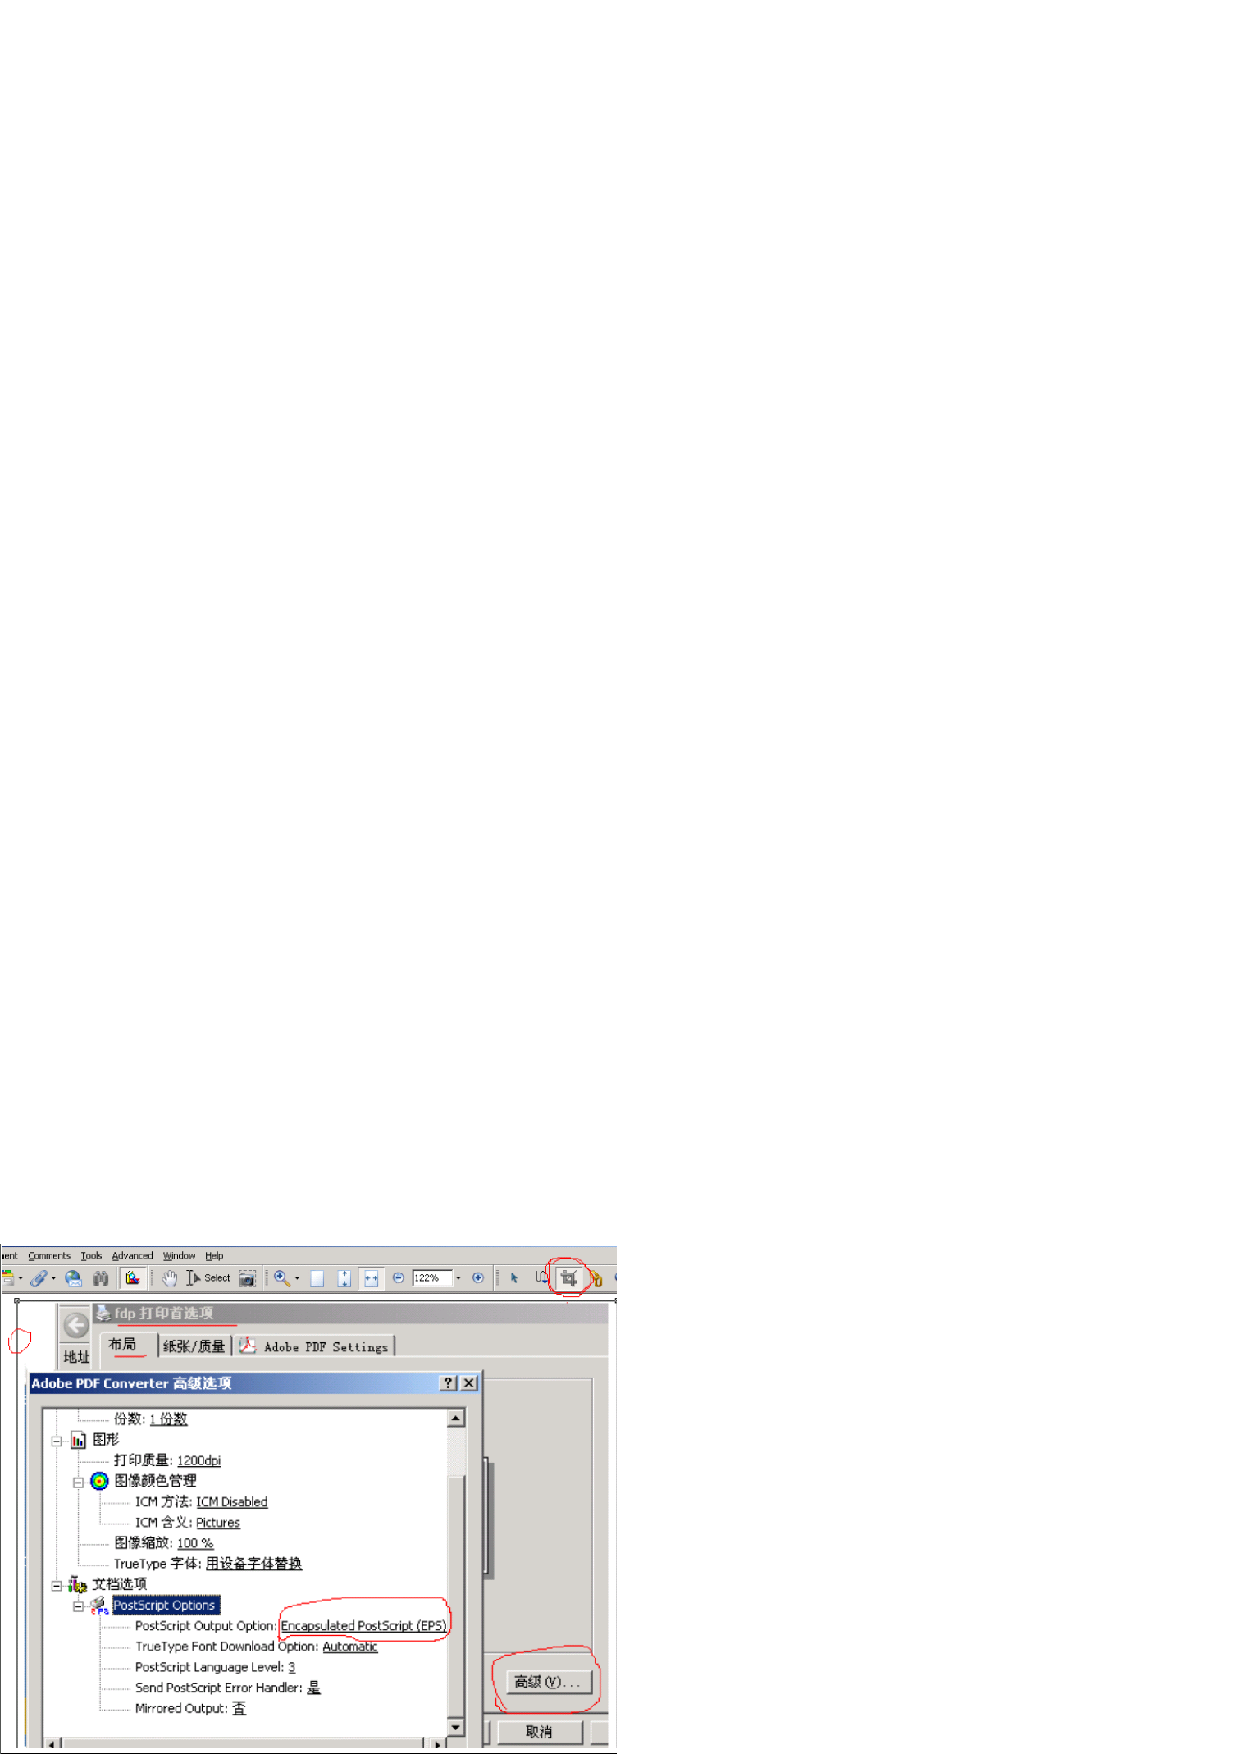
\includegraphics[width = 0.6\textwidth]{get_eps}
\FigCaption{eps ͼ�εĻ��}
\label{Fig:Example1}
\end{figure}

\begin{figure}[htbp]
\centering
\subfigure[�߶���]{\label{Figure:Tricks:Example2:a}
  \includegraphics[width = 0.22\textwidth]{golfer}
}
\subfigure[�߶���]{\label{Figure:Tricks:Example2:B}
  \includegraphics[width = 0.22\textwidth]{golfer}
}
\FigCaption{�߶���}
\label{Fig:Example2}
\end{figure}

\begin{figure}[htbp]
\centering
\begin{minipage}[t]{0.4\textwidth}
\centering
\includegraphics[width = \textwidth]{golfer}\vspace{-5mm}
\FigCaption{��߶��������}
\label{Fig:Example3}
\end{minipage}\hspace{1cm}
\begin{minipage}[t]{0.4\textwidth}
\centering
\includegraphics[width = \textwidth]{golfer}\vspace{-5mm}
\FigCaption{��߶�����}
\label{Fig:Example4}
\end{minipage}
\end{figure}

��~\ref{table:long table}~��һ����ҳ����ʾ����
\begin{longtable}{lll}
\LTCaption{���ı����}\label{table:long table}\\
\bfseries Entity & \bfseries Unicode Name & \bfseries Unicode \\ \hline
\endfirsthead
\bfseries Entity & \bfseries Unicode Name & \bfseries Unicode \\ \hline
\endhead
\hline \multicolumn{3}{r}{\emph{Continued on next page}}
\endfoot
\hline
\endlastfoot
a&emf&bcdef\\
a&emf&bcdef\\
a&emf&bcdef\\
a&emf&bcdef\\
a&emf&bcdef\\
a&emf&bcdef\\
a&emf&bcdef\\
a&emf&bcdef\\
a&emf&bcdef\\
a&emf&bcdef\\
a&emf&bcdef\\
a&emf&bcdef\\
a&emf&bcdef\\
a&emf&bcdef\\
a&emf&bcdef\\
a&emf&bcdef\\
a&emf&bcdef\\
a&emf&bcdef\\
a&emf&bcdef\\
a&emf&bcdef\\
%a&emf&bcdef\\
\end{longtable}

��~\ref{Tricks:Tab1}~��һ����������ӡ�
\begin{table}[htbp]
\centering
\TabCaption{�������}
\label{Tricks:Tab1}
\begin{tabular}{c|c|c}
  \hline
  % after \\: \hline or \cline{col1-col2} \cline{col3-col4} ...
  ���� & ����~(\%) & �ٶ�~(ms) \\
  \hline
  С���任 & $99.8$ &  20\\
  ����Ҷ�任 & $99.0$ & 30 \\
  \hline
\end{tabular}
\end{table}

\subsection{��ʽ}
\label{Tricks:Equations}

�ı��е���ѧ���ź͹�ʽ������ķ������룺

������ѧ��������ȡ��һ���������ģ�;���ͨ����˵��$N$�����⣬����һ
�������£����о������屻�����ʵ㣬$N$��������򵥵ľ��Ƕ������⡣��һ
������ϵͳ�У�$N$��������������$n$���������$k$��С����($N=n+k$)������
$k$��С�������$n$�����������С���Ժ����˶���Ӱ�켸�����ÿ��ǣ���$k$
��С����֮��������Ͻ�������֮����໥����Ӧ�迼�ǣ���͹���������
��($n+k$)�����⡣�ر�أ���$N=3,~n=2,~k=1$ʱ����ͨ����˵���������������⡣


���������ѧ��ʽ������ŵģ�
\begin{equation}
\ddot{\mathbf{r}}=\mathbf{F}_{0}(r)+\mathbf{F}_{\varepsilon}(\mathbf{r},\dot{\mathbf{r}},t)
\end{equation}

����һ��������ŵ����ӣ�
\begin{displaymath}
F_{\varepsilon}/F_{0}=O (\varepsilon)
\end{displaymath}

\FloatBarrier %���������
���͵Ĺ�ʽ�ӷ���˵�������ӣ�

Ŀ���������׷�ٷ�����֮�������˶�����Ϊ��
\begin{equation}\label{eq:1}
\ddot{\boldsymbol{\rho}}-\frac{\mu}{R_{t}^{3}}\left( 3\mathbf{R_{t}}\frac{\mathbf{R_{t}\rho}}{R_{t}^{2}}-\boldsymbol{\rho}\right)=\mathbf{a}
\end{equation}
����

$\boldsymbol{\rho}$---׷�ٷ�������Ŀ�������֮������λ��ʸ����

$\ddot{\boldsymbol{\rho}}$---׷�ٷ�������Ŀ�������֮�����Լ��ٶȣ�

$\mathbf{a}$---�����������ļ��ٶȣ�

$\mathbf{R}_{t}$---Ŀ��������ڹ�������ϵ�е�λ��ʸ����

$\omega_{t}$---Ŀ��������Ĺ�����ٶȣ�

$\mathbf{g}=\frac{\mu}{R_{t}^{3}}\left(
3\mathbf{R_{t}}\frac{\mathbf{R_{t}\rho}}{R_{t}^{2}}-\boldsymbol{\rho}\right)=\omega_{t}^{2}\frac{R_{t}}{p}\left(
3\mathbf{R_{t}}\frac{\mathbf{R_{t}\rho}}{R_{t}^{2}}-\boldsymbol{\rho}\right)$---�������ٶȣ�����$p$��Ŀ��������Ĺ����ͨ����

��ʽ�ӷ���˵��������������
\begin{equation}\label{eq:111}
\ddot{\boldsymbol{\rho}}-\frac{\mu}{R_{t}^{3}}\left( 3\mathbf{R_{t}}\frac{\mathbf{R_{t}\rho}}{R_{t}^{2}}-\boldsymbol{\rho}\right)=\mathbf{a}
\end{equation}
\begin{formulasymb}{ʽ��}{-15pt}%-3pt,-20pt�����Ϸ��ļ�ࡣ
  \fdesfirst{$\boldsymbol{\rho}$}{׷�ٷ�������Ŀ�������֮������λ��ʸ����}
  \fdes{$\ddot{\boldsymbol{\rho}}$}{׷�ٷ�������Ŀ�������֮�����Լ��ٶȣ�}
  \fdes{$\mathbf{a}$}{�����������ļ��ٶȣ�}
  \fdes{$\mathbf{R}_{t}$}{Ŀ��������ڹ�������ϵ�е�λ��ʸ����}
  \fdes{$\omega_{t}$}{Ŀ��������Ĺ�����ٶȣ�}
  \fdes{$\mathbf{g}$}{�������ٶȣ�����$p$��Ŀ��������Ĺ����ͨ����}
\end{formulasymb}

\subsection{�����}{Reference}
ģ����ʹ�õ����϶�������~jdg~�ṩ��~chinesebst.bst��~bib�ļ���д����
����~reference\textbackslash reference.bib��Ҳ��ʹ��EndNote��NoteExpress֮������׹��������Զ����ɡ�
ע�⣬�ڸտ�ʼд����ʱ�����ܰ�~reference.bib ��գ�
�������գ��Ȳ�Ҫ��~bibtex ����,��������~\verb|missing \item| �Ĵ���

��~bst �ļ��������¼�����ɫ��
\begin{hitlist}
  \item �Զ�ʵ�����������е�һ���ʺ�ÿ��ʵ�ʵĵ�һ����ĸ��д������Сд��
  \item ���������߶�������ʱ���Զ�ʶ��������ȡ���������~et al��
  \item ������Ӣ����������������Զ�����ѧλ������ѧУ�����ļ����˳�����⣻
\end{hitlist}

����~\cite{BEZOS02,OOSTRUM01,Zhang2002,zhangsanfeng83} �Ǹ��ݹ�������ҵ��ѧ�����Ĺ淶
��IJο�����ʾ������Ŀ������\citeup{zhangsanfeng,zarchan84}��

\subsection{WinEdt�ı��뼰��������}
\label{sec:winedttricks}
~
��һ�ĵ�~ WinEdt\_LaTeX\_guide.doc �򵥽�����~ WinEdt �ļ��ĵ��ı��뷽�������Ե��
\url{http://bbs.hit.edu.cn/bbscon.php?bid=296&id=1887&ap=719} �õ���

������ϸ���ܱ��밴ť�ĺ��壬����һ�������ر���棬
��ע������Ľ���˳����~ WinEdt ��Ĭ������˳��
\begin{hitlist}
  \item TeX: ��������ʹ��~ TeX ����д���ĵ����ǵײ�ı���ϵͳ��
  \item LaTeX: ��������ʹ��~ LaTeX ����д���ĵ�����Ŀǰ����ʹ������~ LaTeX2e �ĵ�����ϵͳ������~ dvi �ļ���
  \item cct\& LaTeX: cct �ǹ��ڵ����ֲ��о�Ա������һ��ʹ��~ LaTeX �����������ĵ��Ľӿ�ϵͳ��
  ���Ȱ�~cct ���ĵ���~.ctx ת����~.tex ��ʽ��Ȼ����ñ�׼��~ LaTeX ����������dvi�ļ���
  \item PDFLaTeX: ����������~LaTeX������һ�ֱ���ϵͳ��ֱ������~pdf �ļ���֧�ָ����~ pdf �ļ���Ч������Ӧ��Խ��Խ�㷺���������Ļõ�Ƭ��
  \item BibTeX: ��������������ο����׵����ͨ��������һ�������ο�������Ŀ���б�~ bbl �ļ����Ű�ʹ�á�
  \item Make Index: ������������ĵ���������
  \item TeXify: ���Ǽ�����������ĺϼ������Զ�����~ LaTeX����pdflatex����MakeIndex ��~ BibTeX ��������Ҫ�Ĵ���������һ��
  ��������������б��ͽ������õ�~ dvi��pdf���ļ�������~ dvi��pdf���ļ������ɹ��̡�
  \item CTeXify: �����~ CTeX ��װ����������֧�ֵ�~TeXify ��������������ĵ�~ dvi(pdf) �ĵ���
\end{hitlist}

����ʹ���ĸ����밴ť��������ĵ����ͼ������������й�ϵ����Ϊ��ͬ�ı�����������ĵ��е�Ԫ��Ҫ��һ����
���磬��������õ���~eps ͼ�Σ�Ӧ����~latex�����룬����������~pdf ͼ�Σ�Ӧ����~pdflatex �����롣
�����������ǰ����ĵ���Ӧ��Ҳ�Ѿ������ˡ�

\subsection{˶��ѡ��}
��~main.tex~��ע�͵�������伴�ijɲ�ʿģ�塣\\
\verb+\def \xuewei {Master}    % ˶ʿ +

\subsection{���༼�ɼ����������ĵ�}
��������ż��ɣ����Բο��϶���TeX����õ׵�����~\href{http://bbs.hit.edu.cn/bbscon.php?board=TeX&id=2038&ftype=11}{���沿�����⵼��(��Ҫ����������)}��

\subsection{ģ�����Զ����һЩ����}
�������ģ�����Զ����һЩ�����Ҫ���ܣ���ϸ�÷��ɲ���ģ���е�ʾ���ļ�~KaiTi.tex �ȡ�
\begin{hitlist}
\item \verb+\citeup+~����~\verb+\ucite+���������ϱ���ʽ���òο����ף�\verb+\cite+~�������÷�ʽ
\item ͼ�����\verb+\FigCaption, \LTCaption, \TabCaption+
\item ������1����ʽ����~formulasymb��2������빫ʽ~flualign��3���б�����~hitlist
\item �������ۺ�~\verb+\cdash+����ѧģʽ������΢��~dx~\verb+\dif+��
\item �����ֺ��������\verb+\normalbiao+��\verb+\wuhaobiao+
\item �ֺ����\verb+\yihao, \erhao, \xiaoer, \sanhao, \xiaosan+\\
\verb+\sihao, \xiaosi, \wuhao, \xiaowu+������Ĭ����������~\verb+defaultfont+
\end{hitlist}

\subsection{Pluto~����ģ��~FAQs}
\noindent \textbf{Q1}��\textcolor{blue}{�ο������б���Ĵ�Сд�����⣬����д�Ĵ�д����ôת��Сд�ˣ�}\\
\textbf{A1}���ο����׵ı����ʵ������ĸ�Զ���д��������ĸСд������һЩ����ʣ����磺
\verb+{IEEEtran \LaTeX}+ Ӧ��д�� \verb+{IEEEtran} {\LaTeX}+��$\lambda$ Ӧ��д��
\verb+{$\lambda$}+��BaTiO3~дΪ\verb+{BaTiO3}+��

\noindent \textbf{Q2}��\textcolor{blue}{��ͼ������~[~��~]~����ʱ�����dz���ѽ}\\
\textbf{A2}������~subfigure~ʱ�������ͼ���⺬��~[~����Ҫ��~\{~��~\}~��Χ������
\verb+$\beta\in{[0,\,\pi]}$+

\noindent \textbf{Q3}��\textcolor{blue}{���ʱ����еĶ��˺͵Ͷ˵�"����"��ô��}\\
\textbf{A3}��ԭ������\verb+\hline+�ĵط���������\verb+\toprule+��������\verb+\bottomrule+��
����\verb+\specialrule{1pt}{0pt}{0pt}+��

\noindent \textbf{Q4}��\textcolor{blue}{��ôͳ�����ĵ�������}\\
\textbf{A4}��һ����������ַ������Թ���������1. dos������ charcnt main.dvi������~$\approx$~ȫ���ַ���~+~�����ַ���/5��
2. ��~.pdf ����Ϊ~.rtf �ļ���Ȼ����~MS Word~��������ͳ�ơ�

\noindent \textbf{Q5}��\textcolor{blue}{�ο����װ�~bib~�ļ��е�����ȫ���г����ˣ���ʹ��Щ����û�����õ�?}\\
\textbf{A5}����main.tex�в���~\verb+\nocite{*}+~,��ȥ����

\noindent \textbf{Q6}��\textcolor{blue}{������������?}\\
\textbf{A6}���������һ������ڡ�\verb+Ӣ��~���+�������ߡ�\verb+��ѧ~���+����ȥ���м��\verb+~+�����ˡ���дʾ����\verb+control��+��\verb+$a=c$��+��

\noindent \textbf{Q7}��\textcolor{blue}{�������������һ�Σ��������ð���}\\
\textbf{A7}�������о���Ժ���ġ����Ĺ淶��������������ǽ���д�����������������������һ�Ρ������Ҫ��
������~format.tex ��Ѱ�����´��룺
\begin{verbatim}
\titleformat{\subsubsection}[runin]{\hei\sf\xiaosi\boldmath}
{\thesubsubsection}{0.5em}{}[\;\;]
\end{verbatim}
����
\begin{verbatim}
\titleformat{\subsubsection}[hang]{\hei\sf\xiaosi}
{\xiaosi\thesubsubsection}{0.5em}{}
\end{verbatim}

\noindent \textbf{Q8}��\textcolor{blue}{ͼ��λ�õ�����?}\\
\textbf{A8}��ͼ����~\LaTeX~�����ڸ����壬~\LaTeX~��������ݳ��ȣ����е����������λ�ã������Ҫ��ͼ����ij��λ��֮ǰȫ���ų�������ʹ��~\verb+\FloatBarrier+����

\section{ģ��������¼}
\subsection{v0.11 ��һ�����������İ汾}
�ڹ�������ҵ��ѧ˶��ʿѧλ����ģ�壨SVN�ֿ�汾150������1.8rc1��Ŀǰδ������1.8rc2֮�䣩�Ļ����ϣ�LaTeX@lilac
�����˹�����о���˶��ʿ���ⱨ��ģ�塣0.11 ���Ƕ�����~2006 ��~5 �¿����һ��~word ������b5ֽ�ͣ�������Ŀǰû���ѷ��ֵ�������ڣ���ӡЧ����~Word ������ࡣ

\subsection{v0.2 �ڶ���ģ��汾}
������ģ��汾����ϵͳ�ڲ�SVN~195 �汾��Ϊ~v0.2���������������汾��ά����Ϊ~LaTeX �� luckyfox�� ���汾�ĸĶ���Ҫ�����¼������档

\subsubsection{bugs����}
\begin{hitlist}
  \item ������``�ο�����''�ĸ�ʽ��
  \item ������ͼ����ʽ�ı�ţ����±��ȥ����
  \item �������ڷ���"˵��"�ļ�࣬��ʱ�������Ҳ���������������졣��һ��~\verb|\hfill| �Զ�����һ�¡�
  \item ���������Ķ��壬�������治��ð�š�
  \item ͼ��Ӣ�ı��� ��д �� ``Fig'' ��Ϊ``Fig.''��
  \item ���� cmap ���������λ�ã���Ӧ miktex 2.5��
\end{hitlist}


\subsubsection{������ǿ}
\begin{hitlist}
  \item ��ԭ��~b5 ֽ�͵Ļ�����������~a4 ֽ�ͣ����û�ѡ���Ƽ�ʹ��~a4 ֽ�͡�a4 �汾�������ֺ��벩ʿ���Ĺ涨һ�£���о�Ȳ�ʿ����Ҫ�󣬿�������Ϊ���ⱨ�治��װ���ɡ�
  \item �ο����µ�˶ʿ������棬�ṩ��˶ʿ�����֧�֡�
  \item �����˶� winedt5.5 ���Զ��������� tree �� gather �е� toc ��֧�֡�
\end{hitlist}


\subsubsection{�ĵ�˵��}
 \begin{hitlist}
   \item ����``ģ��ʹ��˵��''һ�ڵ�λ�ã�
   \item ����ģ��������¼;
 \end{hitlist}

 \subsection{0.2.0.20071101 ��ǰ������ģ��汾}
�淶�汾�š����汾��ά����Ϊ~LaTeX �� luckyfox�� ���汾�ĸĶ���Ҫ�����¼������档

\subsubsection{bugs����}
\begin{hitlist}
  \item ����ͼ�⼰��ͼ�⣬ʹ�����
  \item  �����ο����� ��İ������ ��reference.bib ������edition=\{�ڶ���\}��Ӣ���� edition=\{2nd\}
  \item �����趨��ʽ�������ĵļ�࣬ԭ����12pt���ָ�Ϊ10pt
  \item a4paper ���븱��ʦһ�ͬʱ����~b5paper ��ά��
  \item ������˫���ӡ��ҳü
  \item �±����е���ѧ���������ĺ�Ŀ¼�мӴ֣��ڱ����е���ѧ�����������мӴ֣���Ŀ¼�в��Ӵ�
  \item ���������ֺ����⣬�����б������ݲ�������֡�
\end{hitlist}


\subsubsection{������ǿ}
\begin{hitlist}
  \item ���� a4paper ���� booktabs ����������߱�
  \item ����relsize��������������ʽ�����С������һ������ flualign �����ڹ�ʽ����롣
\end{hitlist}




%参考文献
\defaultfont
\bibliographystyle{chinesebst}
\addtolength{\bibsep}{-0.8 em} \nocite{*}
\bibliography{reference/reference}
\clearpage

\end{document}
